% Created 2023-04-12 Wed 08:36
\documentclass[9pt, b5paaper]{book}
\usepackage{xeCJK}
\usepackage[T1]{fontenc}
\usepackage[scaled]{beraserif}
\usepackage[scaled]{berasans}
\usepackage[scaled]{beramono}
\usepackage{graphicx}
\usepackage{xcolor}
\usepackage{multirow}
\usepackage{multicol}
\usepackage{float}
\usepackage{textcomp}
\usepackage{geometry}
\geometry{left=1.2cm,right=1.2cm,top=1.5cm,bottom=1.2cm}
\usepackage{algorithm}
\usepackage{algorithmic}
\usepackage{latexsym}
\usepackage{natbib}
\usepackage{minted}
\newminted{common-lisp}{fontsize=\footnotesize}
\usepackage[xetex,colorlinks=true,CJKbookmarks=true,linkcolor=blue,urlcolor=blue,menucolor=blue]{hyperref} 
\author{deepwaterooo}
\date{\today}
\title{dfs}
\hypersetup{
  pdfkeywords={},
  pdfsubject={},
  pdfcreator={Emacs 28.2 (Org mode 8.2.7c)}}
\begin{document}

\maketitle
\tableofcontents


\chapter{dfs 记忆化搜索}
\label{sec-1}
\subsection{1977. Number of Ways to Separate Numbers - Hard}
\label{sec-1-0-1}
You wrote down many positive integers in a string called num. However, you realized that you forgot to add commas to seperate the different numbers. You remember that the list of integers was non-decreasing and that no integer had leading zeros.

Return the number of possible lists of integers that you could have written down to get the string num. Since the answer may be large, return it modulo 109 + 7.
\begin{enumerate}
\item 动态规划: 与最长公共前缀
\label{sec-1-0-1-1}

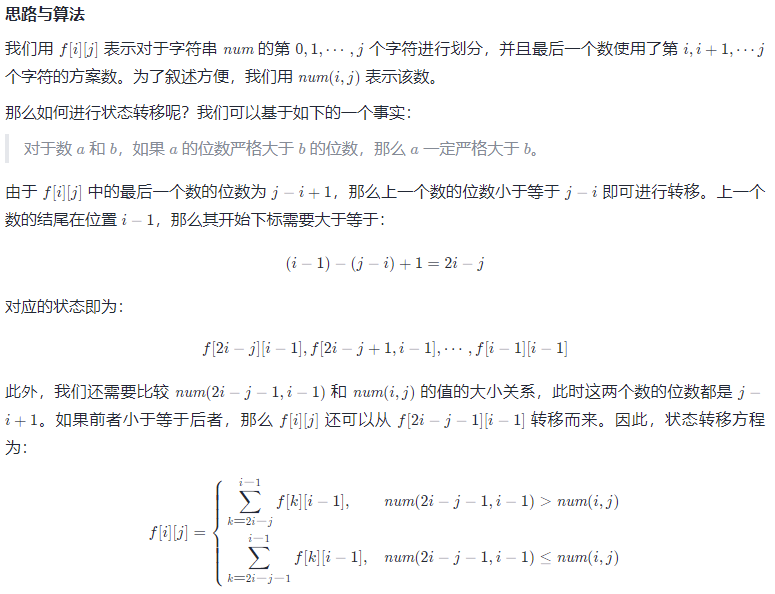
\includegraphics[width=.9\linewidth]{./pic/1977-1.png}

需要注意的是:为了防止状态转移方程显得过于复杂,我们在状态转移方程中:

没有考虑2i−j 和 2i−j−1 是否超出边界。但在实际的代码编写中,需要保证求和式中 kk 的最小值不能小于 00;

没有考虑 num(i,j) 是否包含前导零。如果num[i]=0,那么f[i][j]=0。特别地,如果num\footnote{DEFINITION NOT FOUND.}=0,那么不会有任何满足要求的划分方案,直接返回 00 作为答案,无需进行动态规划。

动态规划的边界条件为 f\footnotemark[1]{}[..] = 1其余的状态的初始值均为 00。最终的答案即为所有 f[..][n - 1]f[..][n−1] 的和,其中 nn 是字符串 num\}num 的长度。

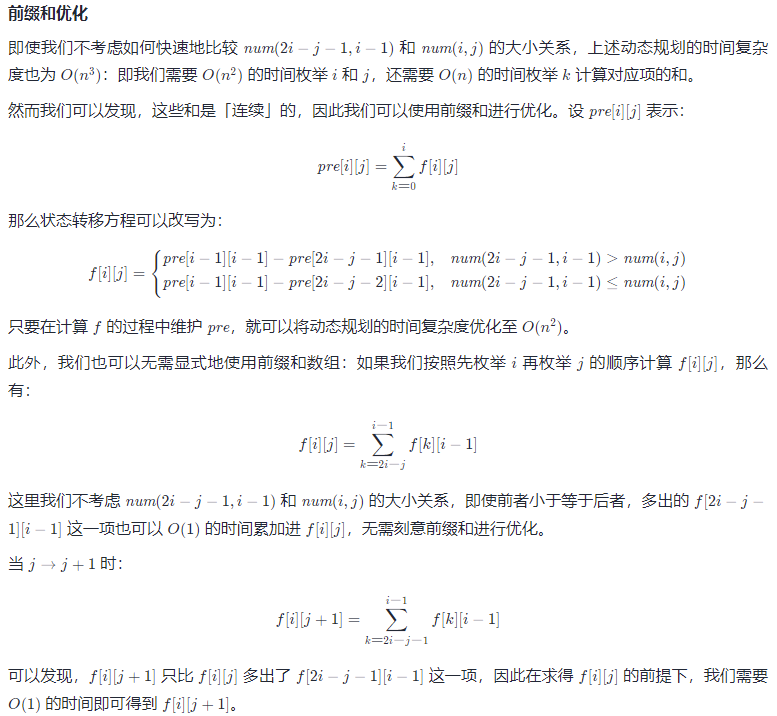
\includegraphics[width=.9\linewidth]{./pic/1977-2.png}

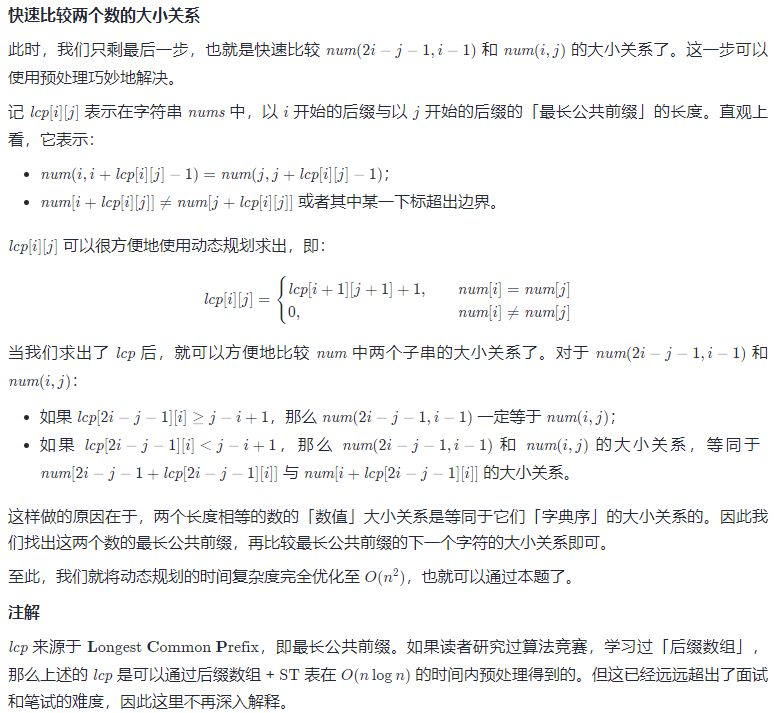
\includegraphics[width=.9\linewidth]{./pic/1977-3.png}

\begin{minted}[fontsize=\scriptsize,linenos=false]{csharp}
static final int mod = (int)1e9 + 7;
public int numberOfCombinations(String t) {
    int n = t.length();
    char [] s = t.toCharArray();
    if (s[0] == '0') return 0;
    int [][] lcp = new int [n][n];   // 求的是: 以s[i]开始的后缀,与以s[j]开始的后缀,两字符串的最长公共前缀长度
    for (int i = n-1; i >= 0; i--) { // 预处理 lcp
        lcp[i][n-1] = s[i] == s[n-1] ? 1 : 0;
        for (int j = i+1; j < n-1; j++) 
            lcp[i][j] = s[i] == s[j] ? lcp[i+1][j+1] + 1 : 0;
    }
    int [][] dp = new int [n][n];
    for (int i = 0; i < n; i++) dp[0][i] = 1; // dp[0][...] = 1
    for (int i = 1; i < n; i++) {
        if (s[i] == '0') continue; // 有前导零,无需转移
        int preSum = 0;
        for (int j = i; j < n; j++) {
            int length = j - i + 1; // s[i,j]
            dp[i][j] = preSum;      // dp[i][j] = d[i][j-1] + (one item) // 这里是j 从 i开始累加的dp[...]前缀和
            if (i - length >= 0) {  // 使用 lcp 比较 s[2i-j-1,i-1] 与 s[i,j] 的大小关系
                if (lcp[i-length][i] >= length || s[i - length + lcp[i-length][i]] < s[i + lcp[i-length][i]])
                    dp[i][j] = (dp[i][j] + dp[i-length][i-1]) % mod;
                preSum = (preSum + dp[i-length][i-1]) % mod; // 更新前缀和,这里是 j 从 i 开始累加的dp[...]前缀和
            }
        }
    }
    int ans = 0;
    for (int i = 0; i < n; i++) // 最终答案即为所有 dp[..][n-1] 的和
        ans = (ans + dp[i][n-1]) % mod;
    return ans;
}
\end{minted}
\begin{itemize}
\item 另一种写法
\end{itemize}
\begin{minted}[fontsize=\scriptsize,linenos=false]{csharp}
private void getLongestCommonPrefixLength() { // Pre compute Longest Common Prefix sequence for each index in the string
    for (int i = n-1; i >= 0; i--)            // 从右向左遍历,计算最长公共前缀序列长度
        for (int j = n-1; j >= 0; j--) 
            if (s[i] == s[j]) {
                if (i >= n-1 || j >= n-1) lcp[i][j] = 1;
                else lcp[i][j] = lcp[i+1][j+1] + 1;
            } else lcp[i][j] = 0;
}
private boolean compare(int i, int j, int len) { // compare substring of same length for value, 
    int commonLength = lcp[i][j];                // 返回以i开始长度为len的序列 是否 比以j开始长度为len的序列(数值)小
    if (commonLength >= len) return true;
    return  s[i + commonLength] <= s[j + commonLength]; // <= ? 为什么不可以等于呢?
}
long mod = (int)1e9 + 7;
int [][] lcp;
char [] s; 
int n;
public int numberOfCombinations(String t) {
    if (t.charAt(0) == '0') return 0;
    n = t.length();
    this.s = t.toCharArray();
    lcp = new int[n][n];
    int [][] f = new int [n][n];
    int [][] pre = new int [n][n];  // 从右向左的累加和
    getLongestCommonPrefixLength(); // 计算从右向左遍历的最长公共前缀(右边,其实是后缀)
    for (int i = 0; i < n; i++) {
        f[0][i] = 1;
        pre[0][i] = 1;
    }
    for (int j = 1; j < n; j++) { // 跟上面超内存的写法是反着走,这次是从左向右遍历,可是两种方法,为什么就有一个会超内存呢?
        for (int i = 1; i <= j; i++) {
            if (s[i] == '0') {
                f[i][j] = 0;
                // continue;
            } else {
                f[i][j] = pre[i-1][i-1];
                if (i - (j-i+1) >= 0) // 现在长度为 i-j+1 的数,前面是否存在一个同样长度的数,即前一个数的第一个位下标是否 >= 0
                    f[i][j] -= pre[2*i-j-1][i-1];
                if (i - (j-i+1) >= 0 && compare(i-(j-i+1), i, j-i+1)) {
                    f[i][j] = (int)((f[i][j] + pre[i-(j-i+1)][i-1]) % mod);
                    if (i - (j-i+1) - 1 >= 0)
                        f[i][j] -= pre[i-(j-i+1)-1][i-1];
                }
            }
            f[i][j] = (int)((f[i][j] + mod) % mod);
            pre[i][j] = (int)((pre[i-1][j] + f[i][j]) % mod);
        }
    }
    return pre[n-1][n-1];
}
\end{minted}
\begin{enumerate}
\item 解题思路与分析 todo: 其它思路,改天补上
\label{sec-1-0-1-1-1}
\end{enumerate}
\end{enumerate}

\subsection{87. Scramble String - Hard 非常经典:要韧熟于心}
\label{sec-1-0-2}
We can scramble a string s to get a string t using the following algorithm:

If the length of the string is 1, stop.
If the length of the string is > 1, do the following:
Split the string into two non-empty substrings at a random index, i.e., if the string is s, divide it to x and y where s = x + y.
Randomly decide to swap the two substrings or to keep them in the same order. i.e., after this step, s may become s = x + y or s = y + x.
Apply step 1 recursively on each of the two substrings x and y.
Given two strings s1 and s2 of the same length, return true if s2 is a scrambled string of s1, otherwise, return false.
\begin{enumerate}
\item 朴素解法(TLE)
\label{sec-1-0-2-1}
一个朴素的做法根据「扰乱字符串」的生成规则进行判断。

由于题目说了整个生成「扰乱字符串」的过程是通过「递归」来进行。

我们要实现 isScrambleisScramble 函数的作用是判断 s1s1 是否可以生成出 s2s2。

这样判断的过程,同样我们可以使用「递归」来做:

假设 s1s1 的长度为 nn, 的第一次分割的分割点为 ii,那么 s1s1 会被分成 [0, i)[0,i) 和 [i, n)[i,n) 两部分。

同时由于生成「扰乱字符串」时,可以选交换也可以选不交换。因此我们的 s2s2 会有两种可能性:

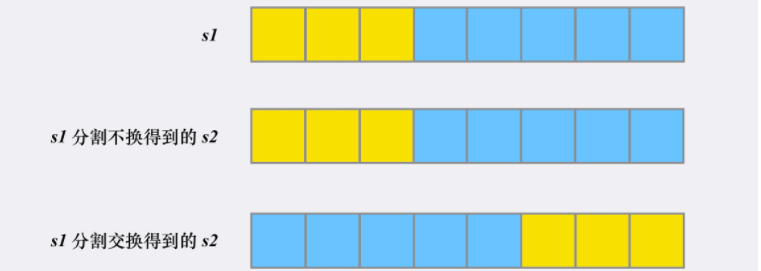
\includegraphics[width=.9\linewidth]{./pic/isScramble.png}


因为对于某个确定的分割点,s1s1 固定分为两部分,分别为 [0,i)[0,i) \& [i, n)[i,n)。

而 s2s2 可能会有两种分割方式,分别 [0,i)[0,i) \& [i,n)[i,n) 和 [0, n-i)[0,n−i) \& [n-i,n)[n−i,n)。

我们只需要递归调用 isScrambleisScramble 检查 s1s1 的 [0,i)[0,i) \& [i, n)[i,n) 部分能否与 「s2s2 的 [0,i)[0,i) \& [i,n)[i,n)」 或者 「s2s2 的 [0, n-i)[0,n−i) \& [n-i,n)[n−i,n)」 匹配即可。

同时,我们将「s1s1 和 s2s2 相等」和「s1s1 和 s2s2 词频不同」作为「递归」出口。

理解这套做法十分重要,后续的解法都是基于此解法演变过来。
\begin{minted}[fontsize=\scriptsize,linenos=false]{csharp}
private boolean idCheck(String ss, String tt) {
    int [] one = new int [26];
    int [] two = new int [26];
    char [] s = ss.toCharArray();
    char [] t = tt.toCharArray();
    for (int i = 0; i < s.length; i++) 
        one[s[i] - 'a']++;
    for (int i = 0; i < t.length; i++) 
        two[t[i]-'a']++;
    for (int i = 0; i < 26; i++) 
        if (one[i] != two[i])
            return false;
    return true;
}
public boolean isScramble(String s, String t) { // tle tle tle
    int n = s.length();
    if (n == 1) return s.charAt(0) == t.charAt(0);
    if (s.equals(t)) return true;
    if (!idCheck(s, t)) return false;
    for (int i = 1; i < n; i++) {
        System.out.println("\n i: " + i);
        String ls = s.substring(0, i), rs = s.substring(i);
        String ltone = t.substring(0, i), rtone = t.substring(i);
        String lttwo = t.substring(0, n-i), rttwo = t.substring(n-i);
        if (isScramble(ls, ltone) && isScramble(rs, rtone)
            || isScramble(ls, rttwo) && isScramble(rs, lttwo))
            return true;
    }
    return false;
}
\end{minted}

时间复杂度:O(5\^{}n)

空间复杂度:忽略递归与生成子串带来的空间开销,复杂度为 O(1)

\item 记忆化搜索
\label{sec-1-0-2-2}
朴素解法卡在了 286 / 288个样例。

我们考虑在朴素解法的基础上,增加「记忆化搜索」功能。

我们可以重新设计我们的「爆搜」逻辑:假设 s1 从 i 位置开始,s2 从 j 位置开始,后面的长度为 len 的字符串是否能形成「扰乱字符串」(互为翻转)。

那么在单次处理中,我们可分割的点的范围为 [1, len),然后和「递归」一下,将 s1 分割出来的部分尝试去和 s2 的对应位置匹配。

同样的,我们将「入参对应的子串相等」和「入参对应的子串词频不同」作为「递归」出口。
\begin{minted}[fontsize=\scriptsize,linenos=false]{csharp}
private boolean idCheck(String ss, String tt) {
    int [] one = new int [26];
    int [] two = new int [26];
    char [] s = ss.toCharArray();
    char [] t = tt.toCharArray();
    for (int i = 0; i < s.length; i++) 
        one[s[i] - 'a']++;
    for (int i = 0; i < t.length; i++) 
        two[t[i]-'a']++;
    for (int i = 0; i < 26; i++) 
        if (one[i] != two[i])
            return false;
    return true;
}
private int dfs(int i, int j, int k) { // k: length dp[i][j][len]: 这个dp的设计还是比较难想的!
    if (dp[i][j][k] != 0) return dp[i][j][k];
    String a = s.substring(i, i+k), b = t.substring(j, j+k);
    if (a.equals(b)) return dp[i][j][k] = 1;
    if (!idCheck(a, b)) return dp[i][j][k] = -1;
    for (int l = 1; l < k; l++) {
        if (dfs(i, j, l) == 1 && dfs(i+l, j+l, k-l) == 1)
            return dp[i][j][k] = 1;
        if (dfs(i, j+k-l, l) == 1 && dfs(i+l, j, k-l) == 1)
            return dp[i][j][k] = 1;
    }
    return dp[i][j][k] = -1;
}
int [][][] dp;
String s, t;
int n;
public boolean isScramble(String s, String t) {
    this.s = s;
    this.t = t;
    n = s.length();
    if (s.equals(t)) return true;
    if (!idCheck(s, t)) return false;
    dp = new int [n][n][n+1];
    return dfs(0, 0, s.length()) == 1;
}
\end{minted}
\item 动态规划(区间 DP)
\label{sec-1-0-2-3}
当然,这道题也可以用动态规划 Dynamic Programming,根据以往的经验来说,根字符串有关的题十有八九可以用 DP 来做,那么难点就在于如何找出状态转移方程。

其实有了上述「记忆化搜索」方案之后,我们就已经可以直接忽略原问题,将其改成「动态规划」了。

根据「dfs 方法的几个可变入参」作为「状态定义的几个维度」,根据「dfs 方法的返回值」作为「具体的状态值」。

我们可以得到状态定义 f[i][j][len]f[i][j][len]:

f[i][j][len]f[i][j][len] 代表 s1s1 从 ii 开始,s2s2 从 jj 开始,后面长度为 lenlen 的字符是否能形成「扰乱字符串」(互为翻转)。

状态转移方程其实就是翻译我们「记忆化搜索」中的 dfs 主要逻辑部分:

\begin{minted}[fontsize=\scriptsize,linenos=false]{csharp}
    // 对应了「s1 的 [0,i) & [i,n)」匹配「s2 的 [0,i) & [i,n)」
    if (dfs(i, j, k) && dfs(i + k, j + k, len - k)) {
        cache[i][j][len] = Y;
        return true;
    }
    // 对应了「s1 的 [0,i) & [i,n)」匹配「s2 的 [n-i,n) & [0,n-i)」
    if (dfs(i, j + len - k, k) && dfs(i + k, j, len - k)) {
        cache[i][j][len] = Y;
        return true;
    }
\end{minted}

从状态定义上,我们就不难发现这是一个「区间 DP」问题,区间长度大的状态值可以由区间长度小的状态值递推而来。

而且由于本身我们在「记忆化搜索」里面就是从小到大枚举 lenlen,因此这里也需要先将 len 这层循环提前,确保我们转移 f[i][j][len] 时所需要的状态都已经被计算好。

这道题看起来是比较复杂的,如果用brute force,每次做切割,然后递归求解,是一个非多项式的复杂度,一般来说这不是面试官想要的答案。

这其实是一道三维动态规划的题目,我们提出维护量res[i][j][n],其中i是s1的起始字符,j是s2的起始字符,而n是当前的字符串长度,res[i][j][len]表示的是以i和j分别为s1和s2起点的长度为len的字符串是不是互为scramble。

有了维护量我们接下来看看递推式,也就是怎么根据历史信息来得到res[i][j][len]。判断这个是不是满足,其实我们首先是把当前s1[i\ldots{}i+len-1]字符串劈一刀分成两部分,然后分两种情况:

第一种是左边和s2[j\ldots{}j+len-1]左边部分是不是scramble,以及右边和s2[j\ldots{}j+len-1]右边部分是不是scramble;

第二种情况是左边和s2[j\ldots{}j+len-1]右边部分是不是scramble,以及右边和s2[j\ldots{}j+len-1]左边部分是不是scramble。

如果以上两种情况有一种成立,说明s1[i\ldots{}i+len-1]和s2[j\ldots{}j+len-1]是scramble的。而对于判断这些左右部分是不是scramble我们是有历史信息的,因为长度小于n的所有情况我们都在前面求解过了(也就是长度是最外层循环)。

上面说的是劈一刀的情况,对于s1[i\ldots{}i+len-1]我们有len-1种劈法,在这些劈法中只要有一种成立,那么两个串就是scramble的。

总结起来递推式是res[i][j][len] = || (res[i][j][k] \&\& res[i+k][j+k][len-k] || res[i][j+len-k][k] \&\& res[i+k][j][len-k]) 对于所有1<=k<len,也就是对于所有len-1种劈法的结果求或运算。因为信息都是计算过的,对于每种劈法只需要常量操作即可完成,因此求解递推式是需要O(len)(因为len-1种劈法)。

如此总时间复杂度因为是三维动态规划,需要三层循环,加上每一步需要线行时间求解递推式,所以是O(n\^{}4)。虽然已经比较高了,但是至少不是指数量级的,动态规划还是有很大有事的,空间复杂度是O(n\^{}3)。

时间复杂度:O(n\^{}4)

空间复杂度:O(n\^{}3)

\begin{minted}[fontsize=\scriptsize,linenos=false]{csharp}
public boolean isScramble(String s, String t) {
    int n = s.length();
    if (s.equals(t)) return true;
    boolean [][][] dp = new boolean [n][n][n+1];
    for (int len = 1; len <= n; len++) 
        for (int i = 0; i+len <= n; i++) 
            for (int j = 0; j+len <= n; j++) {
                if (len == 1) {
                    dp[i][j][len] = s.charAt(i) == t.charAt(j);
                    continue;
                }
                for (int k = 1; k < len; k++) 
                    if (dp[i][j][k] && dp[i+k][j+k][len-k] || dp[i][j+len-k][k] && dp[i+k][j][len-k])
                        dp[i][j][len] = true;
            }
    return dp[0][0][n];
}
\end{minted}
\end{enumerate}

\subsection{2065. Maximum Path Quality of a Graph - Hard 记忆化搜索+ 重复遍历}
\label{sec-1-0-3}
There is an undirected graph with n nodes numbered from 0 to n - 1 (inclusive). You are given a 0-indexed integer array values where values[i] is the value of the ith node. You are also given a 0-indexed 2D integer array edges, where each edges[j] = [uj, vj, timej] indicates that there is an undirected edge between the nodes uj and vj, and it takes timej seconds to travel between the two nodes. Finally, you are given an integer maxTime.

A valid path in the graph is any path that starts at node 0, ends at node 0, and takes at most maxTime seconds to complete. You may visit the same node multiple times. The quality of a valid path is the sum of the values of the unique nodes visited in the path (each node's value is added at most once to the sum).

Return the maximum quality of a valid path.

Note: There are at most four edges connected to each node.
\begin{enumerate}
\item 解题思路与分析
\label{sec-1-0-3-0-1}

A straightforward idea is to try all paths from node 0 and calculate the max path quality for paths also end with node 0.

One \textbf{optimization} we can add is: once we cannot return back to node 0, we stop. The min\_time required from any node to node 0 can be pre-computed using Dijkstra algorithm.

\textbf{Time complexity:} O(4\^{}10)

\textbf{Note the constraints:} 10 <= time\_j, maxTime <= 100 and There are at most four edges connected to each node..

It means the max levels of dfs search is 10, and at each level we have maximum of 4 neighbouring nodes to try.

So the time complexity is: O(4\^{}10).

\begin{minted}[fontsize=\scriptsize,linenos=false]{csharp}
private int [] dijkstra() {
    int [] ans = new int [n];
    Arrays.fill(ans, Integer.MAX_VALUE);
    ans[0] = 0;
    // boolean [] vis = new boolean [n]; // 因为可以重复遍历,要允许它重复遍历  
    // vis[idx] = true;                  // 因为可以重复遍历,要允许它重复遍历  
    // Queue<int []> q = new LinkedList<>();
    Queue<int []> q = new PriorityQueue<>((a, b)->a[1] - b[1]);
    q.offer(new int [] {0, 0});
    while (!q.isEmpty()) {
        int [] cur = q.poll();
        if (cur[1] > ans[cur[0]]) continue;
        for (int [] nei : adj.get(cur[0])) 
            // if (nei[0] == cur[0]) continue; // 因为可以重复遍历,要允许它重复遍历  
            if (nei[1] + cur[1] < ans[nei[0]]) {
                ans[nei[0]] = nei[1] + cur[1];
                // if (!vis[nei[0]]) {
                q.offer(new int [] {nei[0], ans[nei[0]]});
                // vis[nei[0]] = true;
            }
    }
    return ans;
}
private void dfs(int idx, int avaTime, int [] t, int [] v, Set<Integer> vis) {
    if (idx == 0) {
        int cur = 0;
        for (Integer node : vis) 
            cur += v[node];
        ans = Math.max(ans, cur);
    }
    for (int [] nei : adj.get(idx)) 
        if (t[nei[0]] + nei[1] <= avaTime) { //
            boolean added = vis.add(nei[0]);
            dfs(nei[0], avaTime - nei[1], t, v, vis);
            if (added)
                vis.remove(nei[0]);
        }
}
int [] time;
List<List<int []>> adj = new ArrayList<>();
int n, ans = 0;
public int maximalPathQuality(int[] values, int[][] edges, int maxTime) {
    n = values.length;
    for (int i = 0; i < n; i++) 
        adj.add(new ArrayList<>());
    for (int [] e : edges) {
        adj.get(e[0]).add(new int [] {e[1], e[2]});
        adj.get(e[1]).add(new int [] {e[0], e[2]});
    }
    time = dijkstra();
    Set<Integer> si = new HashSet<>();
    si.add(0);
    dfs(0, maxTime, time, values, si);
    return ans;
}
\end{minted}
\end{enumerate}

\subsection{1397. Find All Good Strings - Hard 记忆化搜索}
\label{sec-1-0-4}
Given the strings s1 and s2 of size n and the string evil, return the number of good strings.

A good string has size n, it is alphabetically greater than or equal to s1, it is alphabetically smaller than or equal to s2, and it does not contain the string evil as a substring. Since the answer can be a huge number, return this modulo 109 + 7.
\begin{enumerate}
\item 解题思路与分析: 记忆化搜索
\label{sec-1-0-4-0-1}

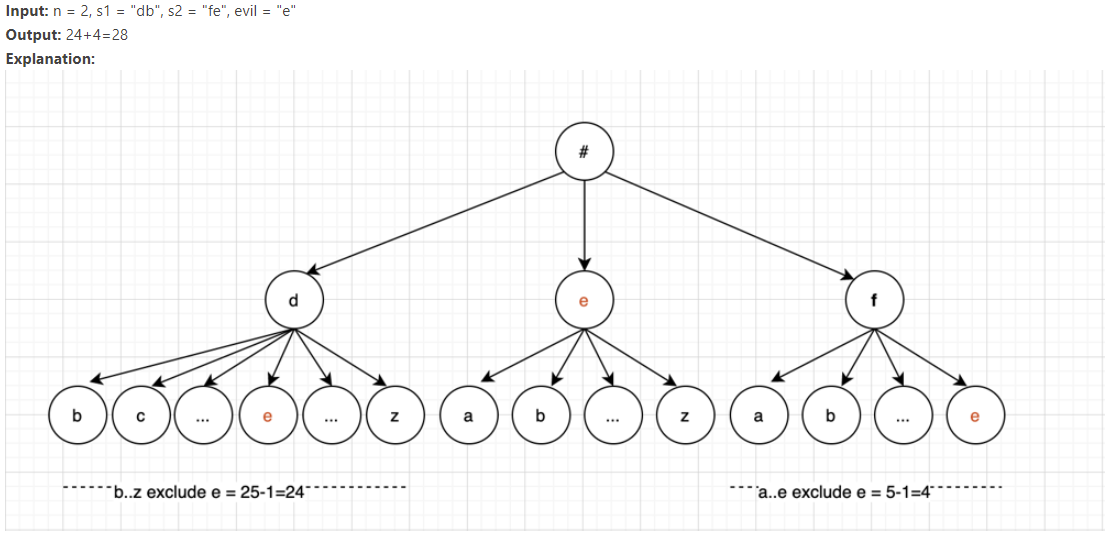
\includegraphics[width=.9\linewidth]{./pic/goodString.png}

\begin{itemize}
\item Complexity
\end{itemize}

Time: O(n*m*2*2*26), where n<=500, m<=50 is length of evil

Space: O(m*n*2*2)

\begin{minted}[fontsize=\scriptsize,linenos=false]{csharp}
private int [] computeLongestPrefixSuffix (char [] s) { // 这个要再理解一下: 重中之重
    int n = s.length;
    int [] lps = new int [n];
    for (int i = 1, j = 0; i < n; i++) {
        while (j > 0 && s[i] != s[j]) j = lps[j-1];  // 转向它 j 的前一位字符(在 j-1 下标)所指向的匹配位置 lps[j-1]
        if (s[i] == s[j]) lps[i] = ++j; // 同时增加两个的下标     
    }
    return lps;
}
private int getKey(int i, int j, boolean l, boolean r) { // bits occupied: i 9, j 6, l 1, r 1
    // 9 bits store n (2^9=512), 6 bits for m (2^6=64), 1 bit ro b1, 1 bit for b2
    return (i << 8) | (j << 2) | ((l ? 1 : 0) << 1) | (r ? 1 : 0); // 这是一个压缩空间存key的聪明技巧
} 
private int dfs(int n, int i, int evilMatched, boolean leftBound, boolean rightBound) {
    if (evilMatched == e.length) return 0; // matched evil string, no good
    if (i == n) return 1;                  // DIDN'T match evil string, great
    int key = getKey(i, evilMatched, leftBound, rightBound); // state: represented by <= 17 bits integer
    if (dp[key] > 0) return dp[key];
    char from = leftBound ? s[i] : 'a';
    char to = rightBound ? t[i] : 'z';
    int ans = 0;
    for (char c = from; c <= to; c++) { 
        int j = evilMatched; // j means the next match between current string (end at char `c`) and `evil` string
        while (j > 0 && e[j] != c) j = lps[j-1]; // 向左回塑寻找match字符c的上一个位置 ?
        if (c == e[j]) j++;
        ans += dfs(n, i+1, j, leftBound && (c == from), rightBound && (c == to));
        ans %= mod;
    }
    return dp[key] = ans;
}
int mod = (int)1e9 + 7;
char [] s, t, e;
int [] dp, lps;
public int findGoodStrings(int n, String s1, String s2, String evil) {
    dp = new int [1 << 17]; // Need total 17 bits, according to data limits
    s = s1.toCharArray();
    t = s2.toCharArray();
    e = evil.toCharArray();
    lps = computeLongestPrefixSuffix(e);
    return dfs(n, 0, 0, true, true);
}
\end{minted}
\item 动态规划: 数位DP + KMP todo: 改天把这个补上
\label{sec-1-0-4-1}
\begin{itemize}
\item \url{https://leetcode-cn.com/problems/find-all-good-strings/solution/shu-wei-dp-kmp-by-qodjf/}
\item \url{https://www.cnblogs.com/wenruo/p/12616985.html}
\item \url{https://www.codeleading.com/article/42703213478/}
\item \url{https://leetcode-cn.com/problems/find-all-good-strings/solution/shu-wei-dp-kmpqian-zhui-shu-zu-java-by-henrylee4/}
\item \url{https://leetcode-cn.com/problems/find-all-good-strings/solution/kmpshang-de-dpc-by-zhu-mang-4/}
\end{itemize}

之前做的题大部分是关于数字的数位dp,而现在要的就是字符串的数位dp。

设d p [ p o s ] [ s t a t s ] [ b o u n d ] dp[pos][stats][bound]为数位dp的数组,其中 p o s pospos表示第pos个位置的字符总共有的数量,s t a t s表示的是匹配e v i l的状态,即能够匹配到e v i l 数组的位置。b o u n d 表示此时能够选择字符的范围,即当前字符选择的时候是否有限制。

对于b o u n d 我们用四个数字表示
\begin{minted}[fontsize=\scriptsize,linenos=false]{csharp}
0 00 表示此时的字符选择是没有限制的,即可以选择的范围为a ∼ z
1 11 表示此时的字符选择是有下限的,所以选择的范围是s 1 [ p o s ] ∼ z
2 22 表示此时的字符选择是有上限的,所以可以选择的范围是a ∼ s 2 [ p o s ]
3 33 表示此时的字符既有上限又有下限。这种情况只有当s 1 [ p o s ] ∼ s 2 [ p o s ]
\end{minted}

而对于stats表示匹配e v i l evilevil字符的状态,由于e v i l evilevil的长度最长为50,所以可以生成字符串e v i l evilevil的next数组。那么当匹配不成立的时候,就可以直接进行跳转。

设一个记忆数组mem[e\_pos][n\_char]表示当匹配e v i l evilevil的位置为e\_pos时,下一个字符为n\_char时,可以跳转的位置,因为在整个搜索的过程中,可能需要多次调用这个数组,而这个数组大小为mem$\backslash$footnote\{DEFINITION NOT FOUND.\}$\backslash$textsuperscript\{,\}$\backslash$,\footnote\{DEFINITION NOT FOUND.\},因此没必要每次都计算。

对于如何生成next的数组,小伙伴们可以去搜索与K M P KMPKMP算法相关的博客查看。
\end{enumerate}

\subsection{2060. Check if an Original String Exists Given Two Encoded Strings - Hard dfs记忆化搜索}
\label{sec-1-0-5}
An original string, consisting of lowercase English letters, can be encoded by the following steps:

Arbitrarily split it into a sequence of some number of non-empty substrings.
Arbitrarily choose some elements (possibly none) of the sequence, and replace each with its length (as a numeric string).
Concatenate the sequence as the encoded string.
For example, one way to encode an original string "abcdefghijklmnop" might be:

Split it as a sequence: ["ab", "cdefghijklmn", "o", "p"].
Choose the second and third elements to be replaced by their lengths, respectively. The sequence becomes ["ab", "12", "1", "p"].
Concatenate the elements of the sequence to get the encoded string: "ab121p".
Given two encoded strings s1 and s2, consisting of lowercase English letters and digits 1-9 (inclusive), return true if there exists an original string that could be encoded as both s1 and s2. Otherwise, return false.

Note: The test cases are generated such that the number of consecutive digits in s1 and s2 does not exceed 3.
\begin{enumerate}
\item 解题思路与分析- (这里需要再好好总结一下)
\label{sec-1-0-5-1}
\begin{itemize}
\item solution is straight forward we have 2 pointer in each string
\end{itemize}
\begin{minted}[fontsize=\scriptsize,linenos=false]{csharp}
1.consider the easy case, they all character, we compare s1.charAt(i) == s2.charAt(j)
2.digit case, we get a number from s1, we can calculate the number s1 has, (descripton said less than 1000), 
  we can pass this value compare with number from s2 name it diff
3.character case if we still has remaing diff to spend passed from our parents, 
  so we can use one dollor a day, one diff one position dfs(i + 1, j, diff - 1
4.terminating condition, if both reach the end and diff == 0
\end{minted}

\begin{minted}[fontsize=\scriptsize,linenos=false]{csharp}
public boolean possiblyEquals(String ss, String tt) {
    m = ss.length(); N = 1000;
    n = tt.length();
    s = ss.toCharArray();
    t = tt.toCharArray();
    dp = new Boolean [m+1][n+1][2001]; // dp[i][j][diff] means if s1[i:] truncated by <diff> characters if diff > 0 
    return dfs(0, 0, 0);               // and s2[j:] truncated by <-diff> characters if diff < 0 are equal
}
Boolean [][][] dp;
char [] s, t;
int m, n, N;
private boolean dfs(int i, int j, int k) { // k: dif
    if (i == m && j == n) return k == 0;
    if (dp[i][j][k+N] != null) return dp[i][j][k+N];
    if (i < m && j < n && k == 0 && s[i] == t[j] && dfs(i+1, j+1, 0))   // Literal matching on s1[i] and s2[j]
        return dp[i][j][N] = true;
    if (i < m && !Character.isDigit(s[i]) && k > 0 && dfs(i+1, j, k-1)) // Literal matching on s1[i]
        return dp[i][j][k+N] = true;
    if (j < n && !Character.isDigit(t[j]) && k < 0 && dfs(i, j+1, k+1)) // Literal matching on s2[j]
        return dp[i][j][k+N] = true;
    for (int x = i, val = 0; x < m && Character.isDigit(s[x]); x++) {   // Wildcard matching on s1[i]
        val = val * 10 + s[x] - '0';
        if (dfs(x+1, j, k-val)) return dp[i][j][k+N] = true;
    }
    for (int x = j, val = 0; x < n && Character.isDigit(t[x]); x++) {   // Wildcard matching on s2[j]
        val = val * 10 + t[x] - '0';
        if (dfs(i, x+1, k+val)) return dp[i][j][k+N] = true;
    }
    return dp[i][j][k+N] = false;
}
\end{minted}
\end{enumerate}

\subsection{638. Shopping Offers - Medium 记忆化搜索 or 背包动态规划}
\label{sec-1-0-6}
In LeetCode Store, there are n items to sell. Each item has a price. However, there are some special offers, and a special offer consists of one or more different kinds of items with a sale price.

You are given an integer array price where price[i] is the price of the ith item, and an integer array needs where needs[i] is the number of pieces of the ith item you want to buy.

You are also given an array special where special[i] is of size n + 1 where special[i][j] is the number of pieces of the jth item in the ith offer and special[i][n] (i.e., the last integer in the array) is the price of the ith offer.

Return the lowest price you have to pay for exactly certain items as given, where you could make optimal use of the special offers. You are not allowed to buy more items than you want, even if that would lower the overall price. You could use any of the special offers as many times as you want.
\begin{enumerate}
\item 解题思路与分析: 记忆化搜索 List作key
\label{sec-1-0-6-1}
\begin{minted}[fontsize=\scriptsize,linenos=false]{csharp}
// 在java里,List的哈希方式,是将其哈希成开头加个1后的31进制整数,例如对于列表[ 1 , 2 , 3 ],java会将其哈希成31进制下的1123,也就是哈希成
// 1*31^3 + 1 * 32^2 + 2 * 31 + 3 = 30817,而List里判断是否equals,是逐个比较列表里的值,如果值全相等就返回true。
//     所以在记忆化的时候,可以直接把key设为是List类型的。
public int shoppingOffers(List<Integer> p, List<List<Integer>> of, List<Integer> need) {
    n = p.size();
    return dfs(p, of, need);
}
Map<List<Integer>, Integer> dp = new HashMap<>();
int n;
private int dfs(List<Integer> p, List<List<Integer>> of, List<Integer> need) {
    if (dp.containsKey(need)) return dp.get(need);  // 首先检查记忆
    int ans = 0;
    for (int i = 0; i < n; i++) 
        ans += p.get(i) * need.get(i);
    if (ans == 0) return ans; // ? 这里就不需要记忆了?
    for (List<Integer> cur : of) {
        if (cur.get(cur.size()-1) >= ans) continue; // >=
        List<Integer> newNeed = new ArrayList<>();
        for (int i = 0; i < n; i++) {
            if (cur.get(i) > need.get(i)) break;
            newNeed.add(need.get(i) - cur.get(i));
        }
        if (newNeed.size() == need.size()) // 即当前礼包合法
            ans = Math.min(ans, cur.get(cur.size()-1) + dfs(p, of, newNeed));
    }
    dp.put(need, ans);
    return ans;
}
\end{minted}
\item 解题思路与分析: 背包动态规划 todo bug fix
\label{sec-1-0-6-2}

当然此题也可以用背包的递推公式来做记忆化搜索,并且使用状态压缩记录每个物品有多少个。由于最多有6 66种物品,每个物品最多6 66个,所以可以用个6 × 3 6\texttimes{} 36×3位二进制数来表示每个物品有多少个。

\begin{minted}[fontsize=\scriptsize,linenos=false]{csharp}
public int shoppingOffers(List<Integer> price, List<List<Integer>> special, List<Integer> needs) { // todo: rest 6 test cases bug to be fixed
    n = price.size();
    int[][] dp = new int[special.size() + 1][1 << (n * 3)]; // 开一个记忆化数组,dp[i][s]表示如果只考虑前i个套餐的话,要买到s这个状态,至少需要多少花费
    System.out.println("(1 << n*3): " + (1 << n*3));
    for (int [] row : dp) Arrays.fill(row, -1); // 先初始化为-1
    int target = 0; // 求一下needs代表的状态,这里target的最低3位表示的是下标是0的商品要买多少个,以此类推
    for (int i = needs.size() - 1; i >= 0; i--) 
        target = (target << 3) + needs.get(i);
    System.out.println("Integer.toBinaryString(target): " + Integer.toBinaryString(target));
    return dfs(special.size(), target, special, price, dp);
}
int n;
// 返回的是,如果只考虑前count个套餐的话,要达到state这个状态的最小花费(当然单买也是考虑的)
private int dfs(int count, int state, List<List<Integer>> special, List<Integer> price, int[][] dp) {
    // System.out.println("state: " + state);
    // if (state >= (1 << n*3)) return 0;
    if (dp[count][state] != -1) return dp[count][state]; // 如果之前已经算出来过,则直接返回
    if (count == 0) { // 如果一个套餐都不考虑,那就是全单买
        dp[count][state] = 0;
        // 求一下每个商品买多少个,然后累加一下花费
        for (int i = 0; i < n; i++) {
            int c = state >> i * 3 & 7;
            dp[count][state] += c * price.get(i);
        }
        return dp[count][state];
    }
    dp[count][state] = dfs(count - 1, state, special, price, dp); // 考虑不选第count个套餐的情况
    List<Integer> sp = special.get(count - 1);                    // 考虑选第count个套餐的情况
    int nextState = 0; // 存一下考虑完当前套餐后的需求状态
    for (int i = n - 1; i >= 0; i--) { // 逆序遍历是为了方便nextState的计算
        int c = state >> i * 3 & 7;
        // System.out.println("c: " + c);
        if (c < sp.get(i)) { // 小了,说明当前套餐是不能选的,标记为-1并退出循环
            nextState = -1;
            break;
        }
        // System.out.println("(c - sp.get(i)): " + (c - sp.get(i)));
        nextState = (nextState << 3) + c - sp.get(i);
        // System.out.println("Integer.toBinaryString(nextState): " + Integer.toBinaryString(nextState));
    }
    if (nextState != -1)  // 如果当前套餐能选,再算一下选了当前套餐的情况下的最小花费
        dp[count][state] = Math.min(dp[count][state], sp.get(n) + dfs(count, nextState, special, price, dp));
    return dp[count][state];
}
\end{minted}
\end{enumerate}
\subsection{474. Ones and Zeroes - Medium}
\label{sec-1-0-7}
You are given an array of binary strings strs and two integers m and n.

Return the size of the largest subset of strs such that there are at most m 0's and n 1's in the subset.

A set x is a subset of a set y if all elements of x are also elements of y.
\begin{enumerate}
\item 解题思路与分析
\label{sec-1-0-7-1}
\begin{minted}[fontsize=\scriptsize,linenos=false]{csharp}
public int findMaxForm(String[] strs, int m, int p) { // m: 0 p: 1 dfs记忆化搜索
    n = strs.length;
    int [] one = new int [n]; // cnt 1s
    int [] two = new int [n]; // cnt 0s
    int cntOne = 0, cntZero = 0;
    for (int i = 0; i < n; i++) {
        String cur = strs[i];
        cntOne = 0;
        cntZero = 0;
        for (char c : cur.toCharArray()) {
            if (c == '0') cntZero++;
            else cntOne++;
        }
        one[i] = cntOne;
        two[i] = cntZero;
    }
    List<String> l = new ArrayList<>();
   cnt = new ArrayList<>();
    for (int i = 0; i < n; i++) {
        if (one[i] > p || two[i] > m) continue;
        l.add(strs[i]);
        cnt.add(new int [] {two[i], one[i]});
    }
    dp = new int [l.size()][m+1][p+1];
    return dfs(l, 0, m, p);
}
int [][][] dp;
List<int []> cnt;
int n;
private int dfs(List<String> l, int idx, int i, int j) { 
    if (idx >= l.size() || i < 0 || j < 0) return 0;
    if (i == 0 && j == 0) return 0;
    if (dp[idx][i][j] > 0) return dp[idx][i][j];
    int x = i - cnt.get(idx)[0], y = j - cnt.get(idx)[1];
    int ans = x >= 0 && y >= 0 ? 1 : 0;
    return dp[idx][i][j] = Math.max(ans + dfs(l, idx+1, x, y), dfs(l, idx+1, i, j));
 }
\end{minted}
\item 解题思路与分析: DP
\label{sec-1-0-7-2}

DP的写法要熟悉起来

\begin{minted}[fontsize=\scriptsize,linenos=false]{csharp}
public int findMaxForm(String[] strs, int m, int n) {
    int [][] dp = new int [m+1][n+1];
    dp[0][0] = 0;
    for (String s : strs) {
        int one = 0, zoo = 0;
        for (int i = 0; i < s.length(); i++) 
            if (s.charAt(i) == '0') ++ zoo;
            else ++one;
        for (int i = m; i >= zoo; i--) 
            for (int j = n; j >= one; j--) 
                dp[i][j] = Math.max(dp[i][j], dp[i-zoo][j-one] + 1);
    }
    return dp[m][n];
}
\end{minted}
\end{enumerate}
\subsection{1900. The Earliest and Latest Rounds Where Players Compete - Hard}
\label{sec-1-0-8}
There is a tournament where n players are participating. The players are standing in a single row and are numbered from 1 to n based on their initial standing position (player 1 is the first player in the row, player 2 is the second player in the row, etc.).

The tournament consists of multiple rounds (starting from round number 1). In each round, the ith player from the front of the row competes against the ith player from the end of the row, and the winner advances to the next round. When the number of players is odd for the current round, the player in the middle automatically advances to the next round.

For example, if the row consists of players 1, 2, 4, 6, 7
Player 1 competes against player 7.
Player 2 competes against player 6.
Player 4 automatically advances to the next round.
After each round is over, the winners are lined back up in the row based on the original ordering assigned to them initially (ascending order).

The players numbered firstPlayer and secondPlayer are the best in the tournament. They can win against any other player before they compete against each other. If any two other players compete against each other, either of them might win, and thus you may choose the outcome of this round.

Given the integers n, firstPlayer, and secondPlayer, return an integer array containing two values, the earliest possible round number and the latest possible round number in which these two players will compete against each other, respectively.
\begin{enumerate}
\item 解题思路与分析:分析本质不同的站位情况 + 记忆化搜索
\label{sec-1-0-8-1}

本题思维难度较大。其中的有些技巧可能在其它的题目中很少出现。

读者在第一次阅读本题解时,可以多去思考「怎么做」,而尽量不要去思考「为什么要这么做」。

\begin{enumerate}
\item 思路与算法
\label{sec-1-0-8-1-1}

我们可以用 F(n, f, s)F(n,f,s) 表示还剩余 nn 个人,并且两名最佳运动员分别是一排中从左往右数的第 ff 和 ss 名运动员时,他们比拼的最早回合数。

同理,我们用 G(n, f, s)G(n,f,s) 表示他们比拼的最晚回合数。

那么如何进行状态转移呢?

只考虑本质不同的站位情况

如果我们单纯地用 F(n, f, s)F(n,f,s) 来进行状态转移,会使得设计出的算法和编写出的代码都相当复杂。例如我们需要考虑 ff 是在左侧(即从前往后数)、中间(即轮空)还是右侧(即从后往前数),对于 ss 也需要考虑那么多情况,这样状态转移方程就相当麻烦。

我们可以考虑分析出本质不同的站位情况,得到下面的表格:
\begin{center}
\begin{tabular}{llll}
\hline
 & s 在左侧 & s 在中间 & s 在右侧\\
\hline
f 在左侧 & 保持不变 & 保持不变 & 保持不变\\
f 在中间 & 等价于「f 在左侧,s 在中间」 & 不存在这种情况 & 等价于「f 在左侧,s 在中间」\\
f 在右侧 & 等价于「f 在左侧,s 在右侧」 & 等价于「f 在左侧,s 在中间」 & 等价于「f 在左侧,s 在左侧」\\
\hline
\end{tabular}
\end{center}
其正确性在于:

\begin{itemize}
\item F(n, f, s) = F(n, s, f) 恒成立。即我们交换两名最佳运动员的位置,结果不会发生变化;
\item F(n, f, s) = F(n, n+1-s, n+1-f) 恒成立。因为我们会让从前往后数的第 ii 运动员与从后往前数的第 ii 名运动员进行比拼,那么我们将所有的运动员看成一个整体,整体翻转一下,结果同样不会发生变化。
\end{itemize}

我们使用这两条变换规则,就可以保证在 F(n, f, s)F(n,f,s) 中,ff 一定小于 ss,那么 ff 一定在左侧,而 ss 可以在左侧、中间或者右侧。这样我们就将原本的 88 种情况减少到了 33 种情况。

对于 G(n, f, s)G(n,f,s),其做法是完全相同的。

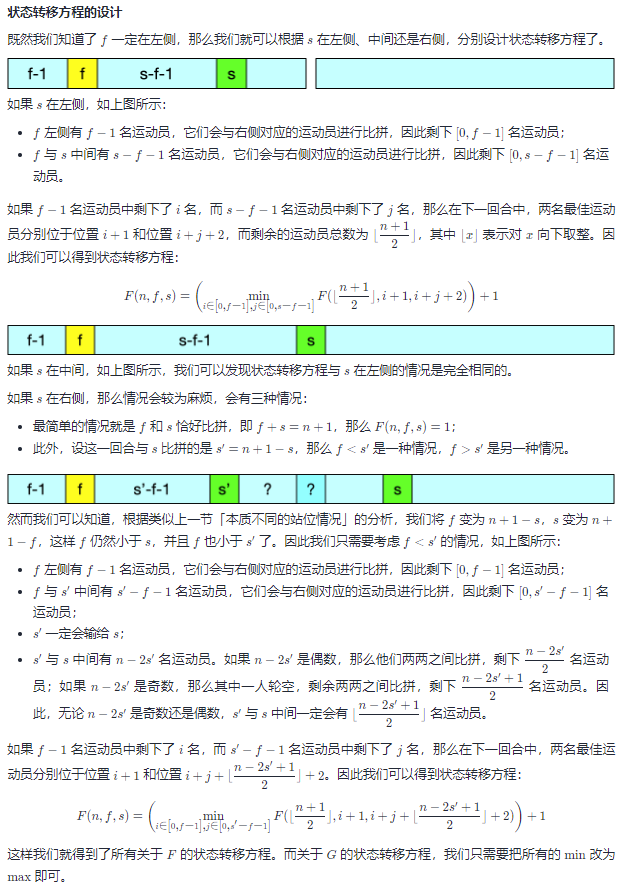
\includegraphics[width=.9\linewidth]{./pic/1900.png}

\item 细节
\label{sec-1-0-8-1-2}

在「本质不同的站位情况」一节中,我们提到了两种变换规则。那么我们具体应当在 n, f, s满足什么关系(而不是抽象的「左侧」「中间」「右侧」)时使用其中的哪些规则呢?

这里有很多种设计方法,我们介绍一种较为简单的,题解代码中使用的方法:

首先我们使用自顶向下的记忆化搜索代替动态规划进行状态转移,这样写更加简洁直观,并且无需考虑状态的求值顺序;

记忆化搜索的入口为 F(n,firstPlayer,secondPlayer)。我们在开始记忆化搜索之前,先通过变换规则 F(n,f,s)=F(n,s,f) 使得firstPlayer 一定小于 secondPlayer,这样一来,由于另一条变换规则 F(n,f,s)=F(n,n+1−s,n+1−f) 不会改变 ff 与 ss 间的大小关系,因此在接下来的记忆化搜索中,f<s 是恒成立的,我们也就无需使用变换规则 F(n,f,s)=F(n,s,f) 了;

在之前表格中,我们需要变换的情况有 55 种,分别是:「ff 在中间,ss 在左侧」「ff 在中间,ss 在右侧」「ff 在右侧,ss 在左侧」「ff 在右侧,ss 在中间」「ff 在右侧,ss 在右侧」。由于我们已经保证了 f < sf<s 恒成立,因此这 55 种情况中只剩下 22 种是需要处理的,即:「ff 在中间,ss 在右侧」和「ff 在右侧,ss 在右侧」。此外,我们在「状态转移方程的设计」一节中还发现了一种需要处理的情况,即「ff 在左侧,ss 在右侧,并且 f> s' =n+1−s」。

那么这 33 种情况是否可以统一呢?对于最后一种情况,我们有 f+s>n+1,而「ff 在中间,ss 在右侧」和「ff 在右侧,ss 在右侧」也恰好满足 f+s > n+1f+s>n+1,并且所有不需要变换的情况都不满足 f+s>n+1。因此我们只需要在 f+s>n+1 时,使用一次变换规则F(n,f,s)=F(n,n+1−s,n+1−f) 就行了。

\begin{minted}[fontsize=\scriptsize,linenos=false]{csharp}
// 3种情况是否可以统一呢?
// 对于最后一种情况,我们有 f+s > n+1f+s>n+1,
// 而「ff 在中间,ss 在右侧」和「ff 在右侧,ss 在右侧」也恰好满足 f+s > n+1f+s>n+1,
// 并且所有不需要变换的情况都不满足 f+s > n+1f+s>n+1。
// 因此我们只需要在 f+s > n+1 时,使用一次变换规则 F(n, f, s) = F(n, n+1-s, n+1-f) 就行
public int [] earliestAndLatest(int n, int firstPlayer, int secondPlayer) {
    min = new int [n+1][n+1][n+1];
    max = new int [n+1][n+1][n+1];
    if (firstPlayer < secondPlayer) return dfs(n, firstPlayer, secondPlayer);
    return dfs(n, secondPlayer, firstPlayer);
}
int [][][] min, max;
private int [] dfs(int n, int f, int s) { // f: firstPlayer, // s: secondPlayer
    if (min[n][f][s] > 0) return new int [] {min[n][f][s], max[n][f][s]};
    if (f + s == n+1) return new int [] {1, 1}; // 刚好第一轮就可以碰上
    if (f + s > n + 1) { // 三种特殊情况的变换:
        int [] res = dfs(n, n+1 - s, n+1 - f);
        min[n][f][s] = res[0];
        max[n][f][s] = res[1];
        return res;
    }
    int glbMin = Integer.MAX_VALUE, glbMax = 0;
    int half = (n+1) >> 1;
    if (s <= half) // // 在左侧或者中间
        for (int i = 0; i < f; i++) // f左侧人数
            for (int j = 0; j < s-f; j++) { // f和s之间的人数
                int [] res = dfs(half, i+1, i+j+2);
                glbMin = Math.min(glbMin, res[0]);
                glbMax = Math.max(glbMax, res[1]);
            }
    else {// s在右侧
        int s_prime = n + 1 - s;
        int mid = (n - 2 * s_prime + 1) / 2;
        for (int i = 0; i < f; i++) 
            for (int j = 0; j < s_prime - f; j++) { // s': n+1-s
                int [] res = dfs(half, i+1, i+j+2 + mid);
                // int [] res = dfs(half, i+1, i+j+2+(s*2-n-1)/2);
                glbMin = Math.min(glbMin, res[0]);
                glbMax = Math.max(glbMax, res[1]); 
            }
    }
    min[n][f][s] = glbMin + 1;
    max[n][f][s] = glbMax + 1;
    return new int [] {glbMin + 1, glbMax + 1};
}
\end{minted}
\end{enumerate}
\end{enumerate}
\subsection{488. Zuma Game - Hard}
\label{sec-1-0-9}
You are playing a variation of the game Zuma.

In this variation of Zuma, there is a single row of colored balls on a board, where each ball can be colored red 'R', yellow 'Y', blue 'B', green 'G', or white 'W'. You also have several colored balls in your hand.

Your goal is to clear all of the balls from the board. On each turn:

Pick any ball from your hand and insert it in between two balls in the row or on either end of the row.
If there is a group of three or more consecutive balls of the same color, remove the group of balls from the board.
If this removal causes more groups of three or more of the same color to form, then continue removing each group until there are none left.
If there are no more balls on the board, then you win the game.
Repeat this process until you either win or do not have any more balls in your hand.
Given a string board, representing the row of balls on the board, and a string hand, representing the balls in your hand, return the minimum number of balls you have to insert to clear all the balls from the board. If you cannot clear all the balls from the board using the balls in your hand, return -1.
\begin{enumerate}
\item 解题思路与分析: bfs广度优先搜索 todo
\label{sec-1-0-9-1}
\begin{minted}[fontsize=\scriptsize,linenos=false]{csharp}
public int findMinStep(String board, String hand) {
    char[] arr = hand.toCharArray();
    Arrays.sort(arr);
    hand = new String(arr);
    // 初始化用队列维护的状态队列:其中的三个元素分别为桌面球状态、手中球状态和回合数
    Queue<State> queue = new ArrayDeque<State>();
    queue.offer(new State(board, hand, 0));
    // 初始化用哈希集合维护的已访问过的状态
    Set<String> visited = new HashSet<String>();
    visited.add(board + " " + hand);
    while (!queue.isEmpty()) {
        State state = queue.poll();
        String curBoard = state.board;
        String curHand = state.hand;
        int step = state.step;
        for (int i = 0; i <= curBoard.length(); ++i) {
            for (int j = 0; j < curHand.length(); ++j) {
                // 第 1 个剪枝条件: 当前球的颜色和上一个球的颜色相同
                if (j > 0 && curHand.charAt(j) == curHand.charAt(j - 1)) 
                    continue;
                // 第 2 个剪枝条件: 只在连续相同颜色的球的开头位置插入新球
                if (i > 0 && curBoard.charAt(i - 1) == curHand.charAt(j)) 
                    continue;
                // 第 3 个剪枝条件: 只在以下两种情况放置新球
                boolean choose = false;
                //  - 第 1 种情况 : 当前球颜色与后面的球的颜色相同
                if (i < curBoard.length() && curBoard.charAt(i) == curHand.charAt(j)) 
                    choose = true;
                //  - 第 2 种情况 : 当前后颜色相同且与当前颜色不同时候放置球
                if (i > 0 && i < curBoard.length() && curBoard.charAt(i - 1) == curBoard.charAt(i) && curBoard.charAt(i - 1) != curHand.charAt(j))
                    choose = true;
                if (choose) {
                    String newBoard = clean(curBoard.substring(0, i) + curHand.charAt(j) + curBoard.substring(i));
                    String newHand = curHand.substring(0, j) + curHand.substring(j + 1);
                    if (newBoard.length() == 0) return step + 1;
                    String str = newBoard + " " + newHand;
                    if (visited.add(str)) 
                        queue.offer(new State(newBoard, newHand, step + 1));
                }
            }
        }
    }
    return -1;
}
public String clean(String s) {
    StringBuffer sb = new StringBuffer();
    Deque<Character> letterStack = new ArrayDeque<Character>();
    Deque<Integer> countStack = new ArrayDeque<Integer>();
    for (int i = 0; i < s.length(); ++i) {
        char c = s.charAt(i);
        while (!letterStack.isEmpty() && c != letterStack.peek() && countStack.peek() >= 3) {
            letterStack.pop();
            countStack.pop();
        }
        if (letterStack.isEmpty() || c != letterStack.peek()) {
            letterStack.push(c);
            countStack.push(1);
        } else countStack.push(countStack.pop() + 1);
    }
    if (!countStack.isEmpty() && countStack.peek() >= 3) {
        letterStack.pop();
        countStack.pop();
    }
    while (!letterStack.isEmpty()) {
        char letter = letterStack.pop();
        int count = countStack.pop();
        for (int i = 0; i < count; ++i) 
            sb.append(letter);
    }
    sb.reverse();
    return sb.toString();
}
class State {
    String board;
    String hand;
    int step;
    public State(String board, String hand, int step) {
        this.board = board;
        this.hand = hand;
        this.step = step;
    }
}
\end{minted}
\item 解题思路与分析: dfs记忆化搜索
\label{sec-1-0-9-2}
\begin{minted}[fontsize=\scriptsize,linenos=false]{csharp}
Map<String, Integer> dp = new HashMap<String, Integer>();
public int findMinStep(String b, String h) {
    char [] s = h.toCharArray();
    Arrays.sort(s);
    h = new String(s);
    int ans = dfs(b, h);
    return ans <= 5 ? ans : -1;
}
private int dfs(String b, String h) {
    if (b.length() == 0) return 0;
    String key = b + "_" + h;
    if (dp.containsKey(key)) return dp.get(key);
    int ans = 6;
    for (int j = 0; j < h.length(); j++) {
        if (j > 0 && h.charAt(j) == h.charAt(j - 1)) continue; // 第 1 个剪枝条件: 当前球的颜色和上一个球的颜色相同
        for (int i = 0; i <= b.length(); ++i) {
            if (i > 0 && b.charAt(i - 1) == h.charAt(j)) continue; // 第 2 个剪枝条件: 只在连续相同颜色的球的开头位置插入新球, 代码不懂 b[i] == b[i-1]?
            boolean choose = false; // 第 3 个剪枝条件: 只在以下两种情况放置新球
            //  - 第 1 种情况 : 当前球颜色与后面的球的颜色相同
            if (i < b.length() && b.charAt(i) == h.charAt(j)) 
                choose = true;
            //  - 第 2 种情况 : 当前后颜色相同且与当前颜色不同时候放置球 (在两个相同着色的中间放置不同着色的球?)
            if (i > 0 && i < b.length() && b.charAt(i - 1) == b.charAt(i) && b.charAt(i - 1) != h.charAt(j)) 
                choose = true;
            if (choose) {
                String newB = clean(b.substring(0, i) + h.charAt(j) + b.substring(i));
                String newH = h.substring(0, j) + h.substring(j + 1);
                ans = Math.min(ans, dfs(newB, newH) + 1);
            }
        }
    }
    dp.put(key, ans);
    return dp.get(key);
}
public String clean(String t) {
    Deque<Character> charSt = new ArrayDeque<Character>();
    Deque<Integer> cntSt = new ArrayDeque<Integer>();
    StringBuffer sb = new StringBuffer();
    char [] s = t.toCharArray();
    for (int i = 0; i < s.length; ++i) {
        char c = s[i];
        while (!charSt.isEmpty() && c != charSt.peek() && cntSt.peek() >= 3) { // 把能消除的先消除掉
            charSt.pop();
            cntSt.pop();
        }
        if (charSt.isEmpty() || c != charSt.peek()) { // 要么栈空了,要么字符不同,入栈(2个)
            charSt.push(c);
            cntSt.push(1); // 记数为1
        } else // 栈顶有相同的字符,但计数不够3,入栈,加数
            cntSt.push(cntSt.pop() + 1);
    }
    if (!cntSt.isEmpty() && cntSt.peek() >= 3) {
        charSt.pop();
        cntSt.pop();
    }
    while (!charSt.isEmpty()) {
        char letter = charSt.pop();
        int count = cntSt.pop();
        sb.append(String.valueOf(letter).repeat(count));
        // for (int i = 0; i < count; ++i) sb.append(letter);
    }
    sb.reverse();
    return sb.toString();
}
class St {
    String b, h;
    int cnt;
    public St(String bd, String hd, int cnt) {
        this.b = bd;
        this.h = hd;
        this.cnt = cnt;
    }
}
\end{minted}
\end{enumerate}
% Emacs 28.2 (Org mode 8.2.7c)
\end{document}